% BASTION masked core, lock-step schedule: architecture figure (Figure 1 in
% the paper). Standalone-compilable: `pdflatex bastion_architecture.tex`
% produces a cropped PDF of the figure alone. To use it inside the paper,
% copy the tikzpicture environment (and the \usetikzlibrary line).
% Revised read-back path: each domain taps both of its banks into its own
% read register (rd0, rd1); the 2:1 output multiplexer sees only those.
\documentclass[tikz,border=4pt]{standalone}
\usetikzlibrary{arrows.meta}
\begin{document}
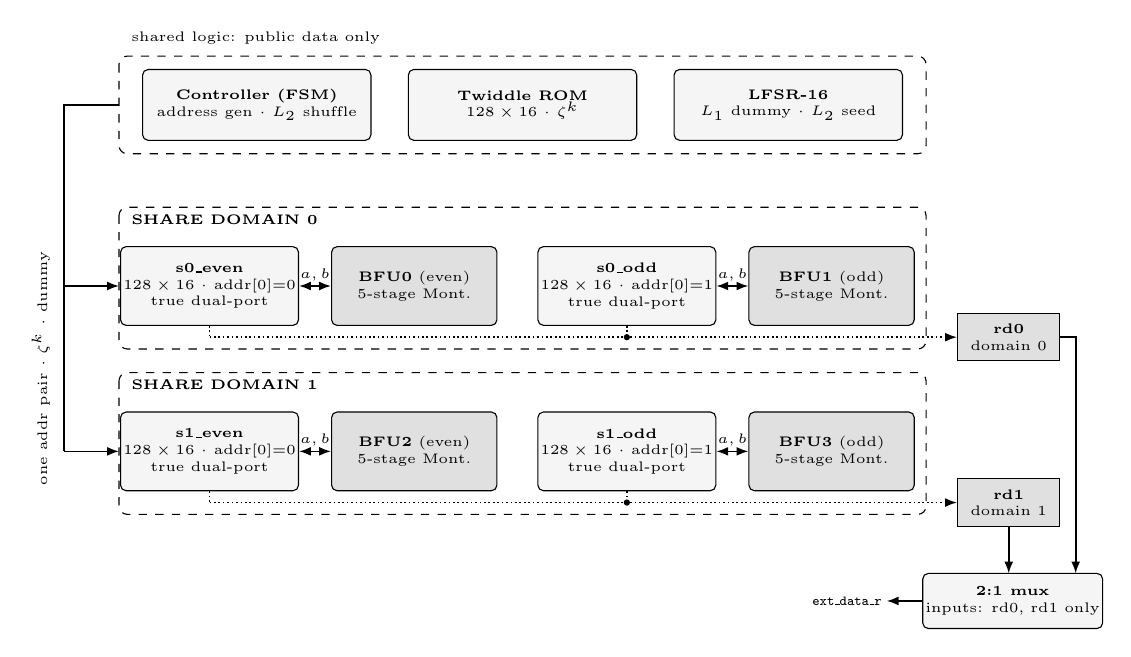
\begin{tikzpicture}[
  x=1cm, y=1cm, font=\sffamily,
  blk/.style={draw, rounded corners=2pt, minimum width=2.1cm,
              minimum height=1.0cm, align=center, inner sep=1pt, font=\tiny},
  mem/.style={blk, fill=black!4},
  bfu/.style={blk, fill=black!12},
  shr/.style={draw, rounded corners=2pt, minimum width=2.9cm,
              minimum height=0.9cm, align=center, inner sep=1pt,
              font=\tiny, fill=black!4},
  reg/.style={draw, minimum width=1.3cm, minimum height=0.6cm,
              align=center, inner sep=1pt, font=\tiny, fill=black!12},
  ar/.style={-{Latex[length=1.5mm]}, semithick},
  dar/.style={-{Latex[length=1.5mm]}, semithick, densely dotted},
  tap/.style={semithick, densely dotted},
  bar/.style={{Latex[length=1.5mm]}-{Latex[length=1.5mm]}, semithick},
  lbl/.style={font=\tiny, inner sep=1.5pt}]

%% shared strip (public data only)
\draw[dashed, rounded corners=3pt] (0,0.62) rectangle (10.25,-0.62);
\node[shr] at (1.75,0)  {\textbf{Controller (FSM)}\\ address gen $\cdot$ $L_2$ shuffle};
\node[shr] at (5.125,0) {\textbf{Twiddle ROM}\\ $128\times16$ $\cdot$ $\zeta^k$};
\node[shr] at (8.50,0)  {\textbf{LFSR-16}\\ $L_1$ dummy $\cdot$ $L_2$ seed};
\node[lbl, anchor=west] at (0.1,0.85) {shared logic: public data only};

%% share domain 0
\draw[dashed, rounded corners=3pt] (0,-1.30) rectangle (10.25,-3.10);
\node[lbl, anchor=north west] at (0.10,-1.34) {\textbf{SHARE DOMAIN 0}};
\node[mem] (b0e) at (1.15,-2.30) {\textbf{s0\_even}\\ $128\times16$ $\cdot$ addr[0]{=}0\\ true dual-port};
\node[bfu] (f0)  at (3.75,-2.30) {\textbf{BFU0} (even)\\ 5-stage Mont.};
\node[mem] (b0o) at (6.45,-2.30) {\textbf{s0\_odd}\\ $128\times16$ $\cdot$ addr[0]{=}1\\ true dual-port};
\node[bfu] (f1)  at (9.05,-2.30) {\textbf{BFU1} (odd)\\ 5-stage Mont.};
\draw[bar] (b0e) -- node[lbl, above]{$a,b$} (f0);
\draw[bar] (b0o) -- node[lbl, above]{$a,b$} (f1);

%% share domain 1
\draw[dashed, rounded corners=3pt] (0,-3.40) rectangle (10.25,-5.20);
\node[lbl, anchor=north west] at (0.10,-3.44) {\textbf{SHARE DOMAIN 1}};
\node[mem] (b1e) at (1.15,-4.40) {\textbf{s1\_even}\\ $128\times16$ $\cdot$ addr[0]{=}0\\ true dual-port};
\node[bfu] (f2)  at (3.75,-4.40) {\textbf{BFU2} (even)\\ 5-stage Mont.};
\node[mem] (b1o) at (6.45,-4.40) {\textbf{s1\_odd}\\ $128\times16$ $\cdot$ addr[0]{=}1\\ true dual-port};
\node[bfu] (f3)  at (9.05,-4.40) {\textbf{BFU3} (odd)\\ 5-stage Mont.};
\draw[bar] (b1e) -- node[lbl, above]{$a,b$} (f2);
\draw[bar] (b1o) -- node[lbl, above]{$a,b$} (f3);

%% public address bus (left)
\draw[semithick] (0,0) -- (-0.70,0) -- (-0.70,-2.30);
\draw[ar] (-0.70,-2.30) -- (0,-2.30);
\draw[semithick] (-0.70,-2.30) -- (-0.70,-4.40);
\draw[ar] (-0.70,-4.40) -- (0,-4.40);
\node[lbl, rotate=90, anchor=south] at (-0.82,-3.35)
      {one addr pair $\cdot$ $\zeta^k$ $\cdot$ dummy};

%% read-back path (right): each domain taps its two banks into its own register
\node[reg] (r0) at (11.30,-2.95) {\textbf{rd0}\\ domain 0};
\node[reg] (r1) at (11.30,-5.05) {\textbf{rd1}\\ domain 1};
\draw[tap] (b0e.south) -- (1.15,-2.95);
\draw[tap] (b0o.south) -- (6.45,-2.95);
\fill (6.45,-2.95) circle (0.04);
\draw[dar] (1.15,-2.95) -- (r0.west);
\draw[tap] (b1e.south) -- (1.15,-5.05);
\draw[tap] (b1o.south) -- (6.45,-5.05);
\fill (6.45,-5.05) circle (0.04);
\draw[dar] (1.15,-5.05) -- (r1.west);
\node[blk, minimum width=1.8cm, minimum height=0.70cm, fill=black!4]
     (mux) at (11.35,-6.30) {\textbf{2:1 mux}\\ inputs: rd0, rd1 only};
\draw[ar] (r0.east) -- (12.15,-2.95) -- (12.15,-5.95);
\draw[ar] (r1.south) -- (11.30,-5.95);
\draw[ar] (mux.west) -- (9.75,-6.30) node[lbl, left]{\texttt{ext\_data\_r}};
\end{tikzpicture}
\end{document}
